\documentclass[11pt]{exam}
\usepackage[spanish]{babel}
\usepackage[utf8]{inputenx}
\usepackage{fontenc}
\usepackage{textcomp}
\usepackage{lmodern,pifont}
\usepackage{graphicx}
\graphicspath{ {./img_/} }
\usepackage{setspace}
\usepackage[dvipsnames]{color}
\usepackage{colortbl}
\usepackage{caption}
\usepackage{amsmath}
\usepackage[normalem]{ulem}

\newcommand\titexam[1]{\centering%
\fbox{\parbox{\textwidth}{\huge \sffamily \textbf{#1}}}\normalsize \vspace{1em}}

\newcommand\materia[1]{%
\parbox{\textwidth}{ \Large \sffamily \textbf{\uline{#1}}}\vspace{1em}}


\newcommand\nombrefecha{%
Nombre y apellidos:\hrulefill
Fecha:\rule{3.5cm}{0.4pt}\vspace{0.5em}}

\renewcommand{\solutiontitle}{\noindent\textbf{Solución:}\par\noindent}
\pagestyle{empty}
\begin{document}
{\fontfamily{lmss}\selectfont

  %%%%%%%%%%%%%%%%%%%%%%%%%%%%%%%%%%%%%
  %% 
\titexam{MF1479\_2 Propagación de plantas en vivero}

\materia{Aspectos básicos de botánica y ecofisiología vegetal}

\nombrefecha
\begin{questions}
  % 1
\question El nombre científico de una especie se forma de dos partes. ¿Puedes
indicar a que categoría taxonómica corresponde la primera parte?
\begin{checkboxes}
  \choice A. Al Reino
  \choice B. A la Familia
  \CorrectChoice C. Al Género
  \choice D. Ninguna es correcta
\end{checkboxes}

\question ¿Sabes que terminación han de tener los taxones pertenecientes a la
categoría de la familia?
\begin{checkboxes}
  \CorrectChoice A. -aceae
  \choice B. -phyta
  \choice C. -ota
  \choice D. La categoría de familia no necesita terminación
\end{checkboxes}

\question Señala cuales de las siguientes especies son coníferas
\begin{checkboxes}
  \choice A. Plataneros, encinas y robles
  \choice B. Pinos, cedros y abetos
  \choice C. Enebros, sabinas y cipreses
  \CorrectChoice D. Las respuestas B y C son correctas
\end{checkboxes}

\question ¿En que categoría generalmente están las plantas que al frotar sus
  hojas, estas desprenden un agradable olor?
  \begin{checkboxes}
    \choice A. Plantas olorosas
    \CorrectChoice B. Plantas aromáticas
    \choice C. Plantas perfumadas
    \choice D. Plantas de rosa
  \end{checkboxes}

\question ¿Qué ecosistemas son extremadamente sensibles a la contaminación por
  plantas invasoras y con las que hay que hay que extremar precauciones?
  \begin{checkboxes}
    \choice A. Ecosistemas de montaña
    \CorrectChoice B. Ecosistemas de agua dulce (ríos y sus
    riveras, lagos, humedales, etc)
    \choice C. Ecosistemas dunares
    \choice D. Ecosistema forestal
  \end{checkboxes}
\newpage
\question ¿Qué tipo de raíz aparece en la imagen?
  \begin{figure}[h!]
    \centering
    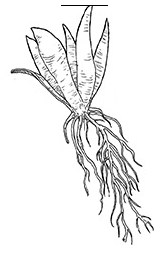
\includegraphics[width=0.2\textwidth]{fasciculada.PNG}
  \end{figure}
  \begin{checkboxes}
    \choice A. Napiforme
    \choice B. Pivotante
    \choice C. Ramificada
    \CorrectChoice D. Fasciculada
  \end{checkboxes}

\question ¿Como se llama la parte del tallo a partir de la cual se pueden
  desarrollar flores o tallos?
  \begin{checkboxes}
    \CorrectChoice A. Yemas
    \choice B. Nudos
    \choice C. Lenticelas
    \choice D. Ninguna respuesta es correcta
  \end{checkboxes}

\question ¿Como se llama la parte que une la hoja con el tallo?
  \begin{checkboxes}
    \choice A. Lamina o limbo
    \choice B. Yema axilar
    \CorrectChoice C. Peciolo
    \choice D. Nervadura
  \end{checkboxes}

\question ¿Como se llama la parte de la flor donde se forma y almacena el polen?
  \begin{checkboxes}
    \choice A. Cáliz
    \CorrectChoice B. Estambre
    \choice C. Tubo polínico
    \choice D. Gineceo
  \end{checkboxes}

\question ¿Cuales son los factores ambientales que influyen en el desarrollo de
  cultivos?
  \begin{checkboxes}
    \CorrectChoice A. Temperatura, radiación e iluminación, altitud, precipitación,
    velocidad del viento
    \choice B. Topografía, orientación, climatología, frió, calor
    \choice C. Temperatura, iluminación
    \choice D. Altitud y precipitaciones
  \end{checkboxes}
\end{questions}
%%%%%%%%%%%%%%%%%%%%%%%%%%%%%%%%%%%%%%%%%%%%%%%%%%%%%%%%%%%%%%%%%%%%%%%%%%%%%%%%%%%%%%%%%%
%%%   PREGUNTAS TEMA 2 %%%%%%%%%%%%%%%%%%%%%%%%%%%%%%%%%%%%%%%%%%%%%%%%%%%%%%%%%%%%%%%%%%%

\titexam{MF1479\_2 Propagación de plantas en vivero}
\materia{Preparación del medio de cultivo}
\nombrefecha
%1
\begin{questions}
\question ¿El suelo se compone principalmente de?
  \begin{checkboxes}
    \choice A. Carbono, nitrógeno y Potasio
    \choice B. Arcilla, arena y limo
    \CorrectChoice C. Minerales de la roca madre, materia orgánica, organismos
    vivos, agua y aire
    \choice D. Roca y organismos vivos
  \end{checkboxes}
%2
\question ¿Como se llaman las capas en las que se divide el suelo para su estudio?
  \begin{checkboxes}
    \CorrectChoice A. Horizontes
    \choice B. Franjas
    \choice C. Capas horizontales
    \choice D. Fronteras
  \end{checkboxes}
%3
\question ¿Qué propiedad física del suelo depende del tamaño de las partículas que la
  componen?
  \begin{checkboxes}
    \CorrectChoice A. Textura
    \choice B. Porosidad
    \choice C. Estructura
    \choice D. Ninguna respuesta es correcta
  \end{checkboxes}
%4
\question ¿Las propiedades del suelo las podemos dividir en?
  \begin{checkboxes}
    \choice A. Físicas, químicas y texturales
    \CorrectChoice B. Físicas, químicas y biológicas
    \choice C. Ph, conductividad eléctrica y capacidad de intercambio catiónico
    \choice D. Las respuestas A y C son correctas
  \end{checkboxes}
%5
\question Los nutrientes de un suelo se clasifican en macroelementos y microelementos. ¿A
  qué se debe el nombre de estos últimos?
  \begin{checkboxes}
    \choice A. A qué la mayoría de elementos son de pequeño tamaño
    \choice B. A qué tienen poca importancia para las plantas
    \choice C. A qué se encuentran en el suelo en poca cantidad
    \CorrectChoice D. A qué se encuentran en las plantas en poca cantidad 
  \end{checkboxes}
% 6
\question Como afecta el pH del suelo a los elementos químicos presentes en el suelo?
  \begin{checkboxes}
    \choice A. Con pH más ácidos la mayoría de los nutrientes serán absorbidos más
    fácilmente
    \choice B. Afecta a la disponibilidad de nutrientes para las plantas.
    \choice C. Dependiendo del pH del suelo algunos nutrientes serán más fácilmente
    absorbidos por las plantas que otros
    \CorrectChoice D. Las respuestas B y C son correctas
  \end{checkboxes}
  % 7
\question El objetivo principal de la preparación de suelos es provocar transformaciones
  que mejoren la germinación y el desarrollo de las plantas. ¿Las preparaciones que se
  realizan pueden conseguir fines como?
  \begin{checkboxes}
    \choice A. Aireación del suelo y/o destrucción de hierbas no deseadas
    \choice B. Aportaciones de nutrientes o enmiendas para mejorar la calidad del suelo
    \choice C. Eliminación de actividad microbiana
    \CorrectChoice D. Las respuestas A y B son correctas
  \end{checkboxes} 
  % 6
\question ¿Qué propiedad física de los suelos relaciona el peso de una materia y
  el volumen que esta ocupa?
  \begin{checkboxes}
    \choice A. Textura
    \CorrectChoice B. Densidad
    \choice C. Porosidad
    \choice D. Tenacidad
  \end{checkboxes}
  % 7
\question Las fertilizaciones en un suelo pueden ser minerales u orgánicas. ¿Qué tipo
  de fertilizantes se emplean en la fertilización orgánica?
  \begin{checkboxes}
    \choice A. Estiércol, humus de lombriz o NPK inorgánico
    \choice B. Abono verde  o enmiendas calizas
    \CorrectChoice C. Estiércol, humus, compost, guano, gallinaza, abono verde
    \choice D. Las respuestas A y B son correctas
  \end{checkboxes}
  % 8
\question ¿La porosidad de un suelo es?
  \begin{checkboxes}
    \choice A. Una propiedad física de los suelos
    \choice B. Una cualidad que determina si el suelo drena en exceso
    \choice C. La relación del volumen de espacios vacíos de un suelo con
    respecto a su volumen total
    \CorrectChoice D. Las respuestas A y C son correctas
  \end{checkboxes}
  % 9
\question Cuando un suelo se encuentra bajo condiciones de exceso de agua
  permanentes y que ponen en peligro los futuros cultivos, ¿qué tipo de
  técnicas se pueden realizar?
  \begin{checkboxes}
    \choice A. Labrado profundo
    \CorrectChoice B. Drenajes
    \choice C. Escardas
    \choice D. Ninguna respuesta es correcta
  \end{checkboxes}
  % 10
\question Si de un suelo decimos que tiene facilidad para que penetre el agua,
  ¿decimos que es un suelo?
  \begin{checkboxes}
    \CorrectChoice A. Permeable
    \choice B. Cohesionado
    \choice C. Estructurado
    \choice D. Ninguna respuesta es correcta 
  \end{checkboxes}
  % 11
\question La frase: \emph{``La ropa de trabajo corriente es un EPI fundamental''}, ¿es?
  \begin{checkboxes}
    \CorrectChoice A. Falsa
    \choice B. Falsa. Solo es un EPI fundamental si los pantalones son largos
    \choice C. Verdadera
    \choice D. Verdadera solo si el operario la utiliza correctamente
  \end{checkboxes}
  % 12
\question ¿Qué consecuencias podría tener un suelo en el que hubiera un exceso
  de poros de gran tamaño?
  \begin{checkboxes}
    \choice A. Que fuese un suelo pesado en el que las raíces se desarrollaran
    con dificultad
    \CorrectChoice B. Un suelo muy suelto que se secase rápidamente
    \choice C. Una labranza dificultosa
    \choice D. Un suelo con una óptima capacidad de retención de agua
  \end{checkboxes}
  % 13
\question ¿Qué propiedad o característica química se relaciona con el contenido
  de sales de un suelo?
  \begin{checkboxes}
    \choice A. El pH
    \choice B. La capacidad de formar otros complejos químicos
    \CorrectChoice C. La conductividad eléctrica
    \choice D. La capacidad de intercambio catiónico
  \end{checkboxes}
  % 14
\question ¿Qué tipo de apero nos permite realizar un labrado vertical?
  \begin{checkboxes}
    \choice A. El arado de vertedera
    \choice B. La grada de discos
    \CorrectChoice C. Con un subsolador o un cultivador
    \choice D. Con un chisel
  \end{checkboxes}
  % 15
\question ¿La vermiculita es un tipo de sustrato?
  \begin{checkboxes}
    \choice A. Un sustrato orgánico
    \CorrectChoice B. Un sustrato inorgánico transformado
    \choice C. Un sustrato de origen natural de origen inorgánico
    \choice D. Ninguna respuesta es correcta 
  \end{checkboxes}
  % 16
\question ¿Los tipos de riesgos que un operario corre por  realizar tareas de abonado del
  terreno pueden ser?
  \begin{checkboxes}
    \choice A. Sobreesfuerzos por manipular cargas o posturas inadecuadas
    \choice B. Contacto con agentes químicos o ingestión accidental de tóxicos
    \choice C. Lesiones en la piel por salpicaduras de residuos o agentes químicos
    \CorrectChoice D. Todas las respuestas son correctas
  \end{checkboxes}
\end{questions}
\newpage
%%%%%%%%%%%%%%%%%%%%%%%%%%%%%%%%%%%%%%%%%%%%%%%%%%%%%%%%%%%%%%%%%%%%%%%%%%%%%%%%%%%%%%%%%%
%%%   PREGUNTAS TEMA 3 %%%%%%%%%%%%%%%%%%%%%%%%%%%%%%%%%%%%%%%%%%%%%%%%%%%%%%%%%%%%%%%%%%%
\titexam{MF1479\_2 Propagación de plantas en vivero}

\materia{Reproducción de plantas por semillas}

\nombrefecha

\begin{questions}
  % 1
\question ¿Como se llama el órgano donde se encuentran las células femeninas en
  la flor?
  \begin{checkboxes}
    \choice A. Gameto
    \CorrectChoice B. Óvulo
    \choice C. Antera
    \choice D. Polen
  \end{checkboxes}
  % 2
\question ¿Qué tipo de ventajas supone la reproducción sexual frente a la
  vegetativa?
  \begin{checkboxes}
    \CorrectChoice A. Aumentar la variación genética de la especie ya que la
    descendencia es producto de los genes de ambos progenitores
    \choice B. Obtener plantas iguales
    \choice C. Que los gametos masculino y femenino se encuentren ya supone 
    un menor gasto energético en la reproducción lo que da como resultado una
    mayor rapidez del proceso
    \choice D. Todas las respuestas son correctas 
  \end{checkboxes}
  % 3
\question ¿La radícula es?
  \begin{checkboxes}
    \choice A. Una parte de una planta
    \choice B. La raíz primordial de una planta que se encuentra en una semilla
    \choice C. Una parte que se encuentra en el embrión de una semilla
    \CorrectChoice D. Las respuestas B y C son correctas
  \end{checkboxes}
  % 4
\question ¿El tegumento o epispermo es una parte de?
  \begin{checkboxes}
    \choice A. De un fruto
    \CorrectChoice B. De una semilla
    \choice C. Es un tipo de polinización
    \choice D. Es la reserva de alimento de una semilla
  \end{checkboxes}
  % 5
\question ¿La acumulación de sustancias de reserva en una semilla se puede dar
  en?
  \begin{checkboxes}
    \choice A. Únicamente en el embrión
    \choice B. En el tegumento
    \CorrectChoice C. En el endospermo o en los cotiledones
    \choice D. Ninguna respuesta es correcta 
  \end{checkboxes}
  % 6
\question Las semillas, según el contenido de humedad que han de retener para
  sobrevivir se clasifican en?
  \begin{checkboxes}
    \CorrectChoice A. Ortodoxas y recalcitrantes
    \choice B. Dehiscentes e indehiscentes
    \choice C. Simples y recalcitrantes
    \choice D. Las respuestas A y C son correctas
  \end{checkboxes}
  % 7
\question ¿La zoocoria es?
  \begin{checkboxes}
    \choice A. Una manera de propagar polen
    \choice B. La dispersión de semillas por el viento
    \choice C. La dispersión de semillas por acción de la gravedad
    \CorrectChoice D. Ninguna respuesta es correcta 
  \end{checkboxes}
  % 8
\question ¿Como se llama una característica propia de las semillas que las impide germinar
  incluso si las condiciones ambientales son favorables?
  \begin{checkboxes}
    \choice A. Vernalización
    \CorrectChoice B. Latencia
    \choice C. Damping-off
    \choice D. Anemocoria
  \end{checkboxes}
\question ¿Qué es un tratamiento pregerminativo de semillas?
  \begin{checkboxes}
    \choice A. Una técnica que mejora la calidad de las semillas
    \CorrectChoice B. Un conjunto de técnicas que han de facilitar el germinado de las
    semillas
    \choice C. Un conjunto de técnicas que aumentan el vigor de las semillas
    \choice D. Todas las respuestas son correctas
  \end{checkboxes}
  % 9
\question ¿Qué es la escarificación?
  \begin{checkboxes}
    \choice A. Una técnica pregerminativa
    \choice B. Alterar la cubierta de las semillas para hacer permeable la semilla
    \choice C. Mediante métodos químicos, físicos o mecánicos modificar el tegumento de
    una semilla
    \CorrectChoice D. Todas las respuestas son correctas 
  \end{checkboxes}
  % 10
\question La época de siembra depende de varios factores. Las coníferas se recomienda que
  se siembren para evitar una enfermedad causada por varios géneros de hongos, ¿denominada?
  \begin{checkboxes}
    \choice A. Vernalización
    \choice B. Latencia
    \CorrectChoice C. Damping-off
    \choice D. Anemocoria    
  \end{checkboxes}
  % 11
\question La competencia originada por hierbas no deseadas puede poner en peligro tanto la
  supervivencia de las semillas como de las plántulas. ¿Como se llama el tratamiento post
  germinativo más que habría que realizar?
  \begin{checkboxes}
    \CorrectChoice A. Escarda
    \choice B. Aclareo
    \choice C. Reposición de marras
    \choice D. Las respuestas A y B son correctas
  \end{checkboxes}
  % 12
\question Además de poder controlar la presencia de hierbas no deseadas de forma manual o
  mecánica, ¿de qué otra manera podemos evitar la presencia de hierbas no deseadas sin
  emplear herbicidas?
  \begin{checkboxes}
    \choice A. Arranque
    \choice B. Siega
    \CorrectChoice C. Mulching o acolchados
    \choice D. Fumigando
  \end{checkboxes}
  % 13
\question ¿La estratificación consiste en?
  \begin{checkboxes}
    \choice A. Un tratamiento pregerminativo
    \choice B. Colocar las semillas embebidas en agua o en estratos húmedos
    \choice C. Alterar el tegumento de las semillas
    \CorrectChoice D. Las respuestas A y B son correctas
  \end{checkboxes}
  % 14 
\question Cuando se realiza la siembra hay que tener especial cuidado con un parámetro que
  puede determinar que la semilla quede expuesta a la desecación y los agentes
  meteorológicos o que la germinación se retrase mucho o no ocurra. ¿Hablamos de?
  \begin{checkboxes}
    \choice A. La época de siembra
    \CorrectChoice B. La profundidad de siembra
    \choice C. La densidad de siembra
    \choice D. Todas las respuestas son correctas
  \end{checkboxes}
  % 15
\question En las operaciones de repicado, ¿qué EPI es imprescindible llevar, especialmente
  si el operario es fumador?
  \begin{checkboxes}
    \choice A. Gafas
    \CorrectChoice B. Guantes de látex
    \choice C. Mascarillas
    \choice D. Guantes de cuero
  \end{checkboxes}
  % 16
\question ¿Como se llama la instalación que está destinada a proteger de la radiación
  solar a los cultivos?
  \begin{checkboxes}
    \choice A. Malla antihierba
    \choice B. Vivero
    \choice C. Manta térmica
    \CorrectChoice D. Ombráculo
  \end{checkboxes}
\end{questions}
%%%%%%%%%%%%%%%%%%%%%%%%%%%%%%%%%%%%%%%%%%%%%%%%%%%%%%%%%%%%%%%%%%%%%%%%%%%%%%%%%%%%%%%%%%
%%%   PREGUNTAS TEMA 4 %%%%%%%%%%%%%%%%%%%%%%%%%%%%%%%%%%%%%%%%%%%%%%%%%%%%%%%%%%%%%%%%%%%

\titexam{MF1479\_2 Propagación de plantas en vivero}
\materia{Reproducción vegetativa}
\nombrefecha
\begin{questions}
  % 1
\question Las plantas tienen capacidad de reproducirse de manera asexual mediante
  ciertas estructuras tales como?
  \begin{checkboxes}
    \CorrectChoice A. Bulbos y tubérculos
    \choice B. Estacas y esquejes
    \choice C. Acodo y rizoma
    \choice D. Todas las respuestas son correctas 
  \end{checkboxes}
  % 2
\question ¿Cuales son las ventajas de la reproducción vegetativa?
  \begin{checkboxes}
    \CorrectChoice A. Mantiene las características de la planta madre, es más
    rápido y ciertos árboles pueden resultar más pequeños
    \choice B. Requiere de mano de obra entrenada y necesita de ciertas
    infrestructuras
    \choice C. No existe variabilidad genética y la longevidad no és mayor que
    en la reproducción sexual
    \choice D. Obtiene plantas diferentes de los progenitores y es más facil de
    conservar 
  \end{checkboxes}
  % 3
\question ¿Como se llama el órgano de reproducción subterráneo que está
  formado por hojas carnosas modificadas?
  \begin{checkboxes}
    \choice A. Tubérculo
    \choice B. Rizoma
    \choice C. Pedúnculo
    \CorrectChoice D. Bulbo
  \end{checkboxes}
  % 4
\question ¿Como se llama el órgano de reproducción subterráneo que está formado
  por un engrosamiento de las raíces?
  \begin{checkboxes}
    \CorrectChoice A. Tubérculo
    \choice B. Rizoma
    \choice C. Estolones
    \choice D. Bulbo    
  \end{checkboxes}
  % 5
\question ¿Cuales de las siguientes especies son ejemplos de bulbos?
  \begin{checkboxes}
    \choice A. Cebolla
    \choice B. Narciso
    \choice C. Tulipán
    \CorrectChoice D. Todas las respuestas son correctas 
  \end{checkboxes}
  % 6
\question ¿Cuantas yemas debe contener como mínimo un esqueje o estaquilla para un correcto
  desarrollo y enraizado?
  \begin{checkboxes}
    \choice A. No importa el número de yemas, solo la calidad de la planta madre
    \choice B. Una
    \CorrectChoice C. Dos
    \choice D. Con una yema será suficiente siempre y cuando dejemos las hojas completasd
  \end{checkboxes}
  % 7
\question ¿Como se llama la técnica de reproducción vegetativa en la que se
  fuerza a un tallo a emitir raíces adventicias?
  \begin{checkboxes}
    \choice A. Injerto
    \CorrectChoice B. Acodo
    \choice C. Estaquillado
    \choice D. Estolonado
  \end{checkboxes}
  % 8
\question ¿Qué es un patrón?
  \begin{checkboxes}
  \choice A. Persona encargada de los trabajos en el campo
  \CorrectChoice  B. Planta que recibe un injerto y aporta el sistema radicular
  \choice C. Trozo de rama que se introduce en un pie o planta para reproducirla
  \choice D. Parte de una rama en la que hacemos una incisión para quitar un
  anillo y que cubrimos con sustrato ayudandonos de una bolsa.
  \end{checkboxes}
  % 9
\question 
\end{questions}

}
\end{document}
%%% Local Variables:
%%% mode: latex
%%% TeX-master: t
%%% End:
